%!TEX encoding = UTF-8 Unicode

\section{Proposed Approach}

We follow the method adopted in the evaluation part of~\cite{salvi:2012:smcb}, however, instead of assuming that the action identities are known to the robot agent, we estimate them by observing an external agent and applying statistical inference methods and \acp{HMM}.

\begin{figure}
  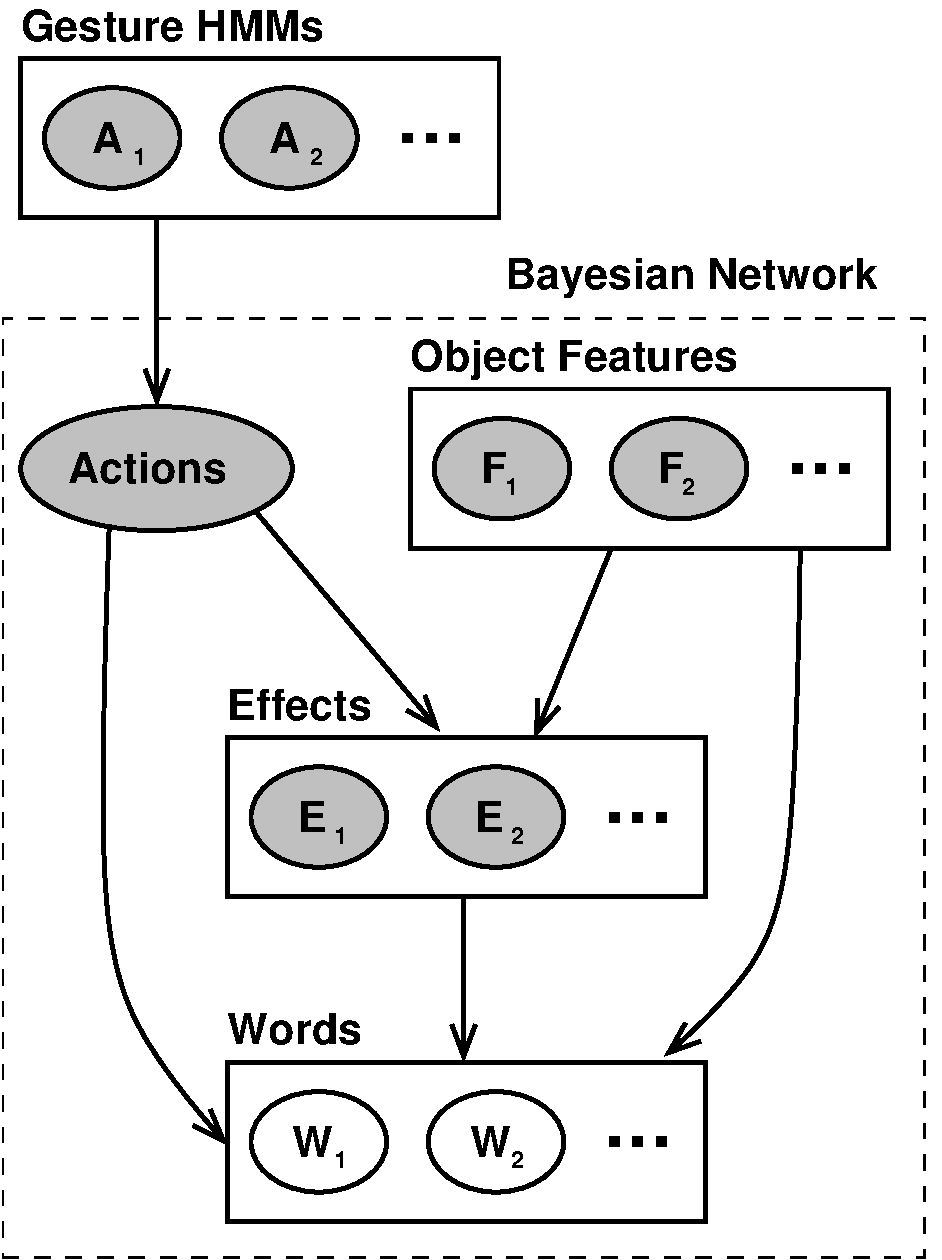
\includegraphics[width=\columnwidth]{fullNetAbstract}
  \caption{Abstract representation of the probabilistic dependencies in the model.}
\end{figure}

In the experimental section, we will show that what the robot has learned subjectively or alone~(by self-exploration, knowing the action identity as a prior~\cite{salvi:2012:smcb}), can subsequently be used when observing a new agent~(human), provided that the actions can be estimated with \acp{HMM} as in~\cite{saponaro:2013:crhri}.
